\graphicspath{{chapters/images/02/}}

\chapter{Second Week}

\section{Central Dogma}

\section{Measure biomolecules}
\textbf{Proteins}
\begin{itemize}
	\item Western blot
	\item ELISA
	\item Northern blot
	\item Enzyme assay
\end{itemize}\\


\textbf{RNA}
\begin{itemize}
	\item \textbf{DNA microarray}: it is an old technique
	\item RT-PCR
	\item \textbf{RNA sequencing} based on next generation sequencing  
\end{itemize}\\

\subsection{DNA microarrays}
points on a glass slide, technology invented in 1990s, they were developed after macroarrays.
The technology can be used to quantify miRNA, SNP excetera. It includes all the genes in the genome, including the splice variants and it is reliable for gene expression quantifications. It is easy to analyze, thanks to the bioinformatics resources that are now available.

\begin{figure}[h]
\caption{}
\centering
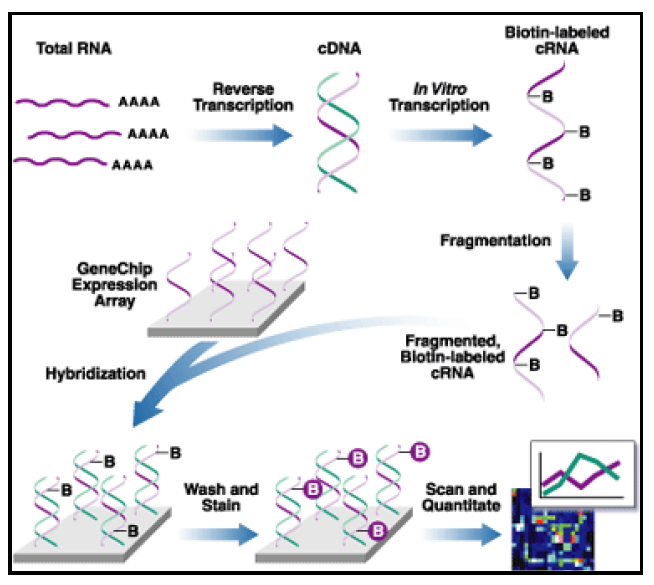
\includegraphics[width=0.6\textwidth]{microarrays}
\end{figure}

Affimetrix is a device that permits to do everything on a chip, it was developed for a series of species\\
Competitor of Affimetrix is Illumina BeadChip, beads are ligated to oligonucleotides. The beads are inside wells. Illumina makes two colours cheaps (in terms of fluorescence). The possible source of errors are depicted in the image:
The first thing to do is to extract RNA from cells, which could be contaminated, then the extraction of RNA occurs, and a low extraction is possible. Degradation of RNA could also happen. During the reverse transcription, and fluorescent labelling, you have to ensure that the reverse transcription happen for each molecule, and each has to be labled. After, during hybridization has to occur equally for all the molecules, it could also happen cross-hybridization. Longer fragments can help in this. Scanning errors could also take place at the end.

\begin{figure}[h]
\caption{}
\centering
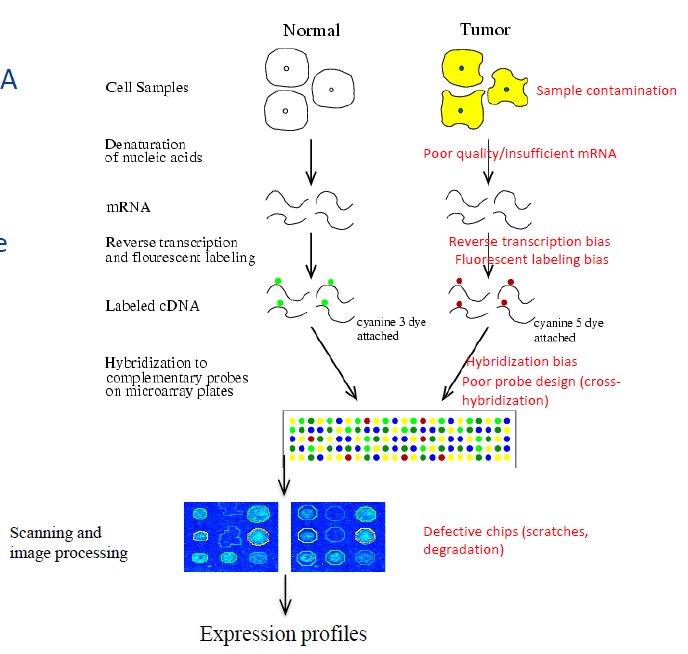
\includegraphics[width=0.6\textwidth]{ProblemsMicarrays}
\end{figure}

Other types of errors, can be due to non-specific fluorescence. Binding could also happen not specifically. Some methods exist to reduce the noise (error), for example: the Affy matrix, which uses two probes, one with Perfect Matches and a similar probe, but with a single different nucleotids (mismatch). If you subtract the two fluorescences, you should eliminate the noisy fluorescence (due to non-specific hybridizations).

At the end, it is obtained an \textbf{absolute quantification}.

